\documentclass[final,hyperref={pdfpagelabels=false}]{beamer}
\usepackage{grffile}
\mode<presentation>{\usetheme{I6pd2}}
\usepackage[english]{babel}
\usepackage[latin1]{inputenc}
\usepackage{amsmath,amsthm, amssymb, latexsym}
%\usepackage{times}\usefonttheme{professionalfonts}  % obsolete
%\usefonttheme[onlymath]{serif}
\boldmath
\usepackage[orientation=portrait,size=a0,scale=1.4,debug]{beamerposter}
\usepackage{ragged2e} 
\usepackage{bm}
% change list indention level
% \setdefaultleftmargin{3em}{}{}{}{}{}

%\usepackage{snapshot} % will write a .dep file with all dependencies, allows for easy bundling


\usepackage{array,booktabs,tabularx}
\newcolumntype{R}{>{\centering\arraybackslash}X} % right justified tabularx columns
\newcommand{\pphantom}{\textcolor{ta3aluminium}} % phantom introduces a vertical space in p formatted table columns??!!
\newcommand{\p}{\partial}
\newcommand{\bu}{\bm{u}}
\newcommand{\bv}{\bm{v}}

\listfiles

%%%%%%%%%%%%%%%%%%%%%%%%%%%%%%%%%%%%%%%%%%%%%%%%%%%%%%%%%%%%%%%%%%%%%%%%%%%%%%%%%%%%%%
\graphicspath{{figures/}}
 
\title{\huge Gap formation and stability in non-isothermal
  disks\\ \Large [2014 CITA Summer Student Program]}
\author{Min-Kai Lin and Robert Les}
\institute[CITA]{Canadian Institute for Theoretical Astrophysics, 60
  St George Street, Toronto, M5S 3H8, Canada}
%% \date[Sep. 8th, 2009]{Sep. 8th, 2009}

%%%%%%%%%%%%%%%%%%%%%%%%%%%%%%%%%%%%%%%%%%%%%%%%%%%%%%%%%%%%%%%%%%%%%%%%%%%%%%%%%%%%%%
\newlength{\columnheight}
\setlength{\columnheight}{105cm}
\setbeamertemplate{caption}{\centering\insertcaption\par}

%%%%%%%%%%%%%%%%%%%%%%%%%%%%%%%%%%%%%%%%%%%%%%%%%%%%%%%%%%%%%%%%%%%%%%%%%%%%%%%%%%%%%%
\begin{document}
\begin{frame}
  \begin{columns}

    %Aspect ratio: For higher $\tilde{\beta}$ values the disk aspect ratio increases non-monotonicly. Values for $\tilde{\beta}=0.1,1.0,10.0$ are $h=0.05,0.055,0.08$. The values are not constant over time and make roughly parabolic shapes from intial planet formation to vortex death. The aspect ratio of the vortices themselves seem to be constantly near $h=0.05$ regardless of the cooling paramter. Also $\tilde{\beta}=5.0$ which has longest lifetime (2000+ orbits) corresponds to approximately $h=0.06$ which is similar result as Fu et al. 

    %Mach Number: Mach numbers generally in the vortex region of disk averaged aziumthally are $<0.4$ during semi-stable vortex state. Just as vortex dies out mach numbers drop to $M=0.2$ which are from the shock. Mach number near vortices during semi-stable state are near 0.2 from 2D plots.
    
    %Reynold's Stress:The averaged reynold's stress of the disk is usually of order $\alpha=10^{-2} - 10^{-3}$. During vortex death $\alpha=10^{-2}$ consistantly for all $\tilde{\beta}$ than drops to lower bound after vortex dissipation. Vortices themselves seem to have almost no characteristic reynolds stress associated with them from 2D plots.

    %Gap profile:After vortex death sees a distortion in outer gap depth and the outer gap edge slowly and continuously extends outwards. Gap edge in semi-steady state is around 5 hill radii (gap edges not very clear since current resolution isn't good). Changes in gap depth start before vortex dissaption and indicate that matter is moving inwards towards the planet. Supports notion that vortex distorts background profile. This effect increases largely during the dissipation phase

    %Vortex:The overdensiy of the vortex itself can reach 10 times the intial density of the disk. Vortex evolves from a large vortex to a highly dense small vortex. As it dies off the vortex distorts in shape most probably from interaction with shocks.Disapation time is around 50 orbits.
    
    %Rossby Numbers:Rossby numbers during semi-stable states are approximately around $Ro=-0.2$. Just after vortex amplitude drop, Rossby numbers increase to around $Ro=-0.4$ because of spreading of angular momentum from the once densly packed spinning vortex.

    %Non-linear Planet off:Long Term planet-off simulations do not show these drops in vortex amplitude. The vortices are of order of magnitude less in max amplitude and over time slowly decay assumingly by viscous friction. This supports fact that planet helps drive the interactions we are seeing. Results in progress.

    % ---------------------------------------------------------%
    % Set up a column 
    \begin{column}{.49\textwidth}
      \begin{beamercolorbox}[center,wd=\textwidth]{postercolumn}
        \begin{minipage}[T]{.95\textwidth}  % tweaks the width, makes a new \textwidth
          \parbox[t][\columnheight]{\textwidth}{ % must be some better way to set the the height, width and textwidth simultaneously
            % Since all columns are the same length, it is all nice and tidy.  You have to get the height empirically
            % ---------------------------------------------------------%
            % fill each column with content            
            \begin{block}{{\Large Introduction}}
              \justifying
                  {\large              
                    {\bf
                    }
                  }
            \end{block}
            \vfill
             
            \begin{block}{{\Large Disk-planet model with simple
                  cooling}}
              \justifying
             We numerically evolve the 2D fluid equations including a
             gap-opening giant planet, treated as an external
             potential on fixed circular orbit. We include in the
             energy equation  
        a simple source term in the form 
	\begin{align*}
	\frac{\partial e}{\partial t} = \cdots + \frac{e-e_{t=0}}{t_\mathrm{cool}},
	\end{align*}
        and $t_\mathrm{cool} = \beta \Omega_k^{-1}$, where $\Omega_k$ is the Keplerian frequency. We choose $\beta$ indirectly 
        through $\tilde{\beta}$ such that
        \begin{align*}
        t_\mathrm{cool, gap\,edge} = \tilde{\beta} t_\mathrm{lib, gap\,edge},
        \end{align*}
        where $t_\mathrm{lib, gap\,edge}$ is the time interval between successive encounters of a fluid element, 
        located at the gap edge, and the planet's azimuth. Thus $\tilde{\beta}\ll 1$ implies that such a fluid returns to its initial temperature
        before passing by the planet again. 
        \end{block}
        \vfill

        \begin{block}{{\Large Planet gaps as a function of cooling
              rate}}
          \justifying
          % {\bf generalized vortensity profile due to planet for
          %   different beta. also density profiles.}
          
          \begin{figure}
            \centering
%            \hfill
%            \begin{minipage}{0.49\textwidth}
              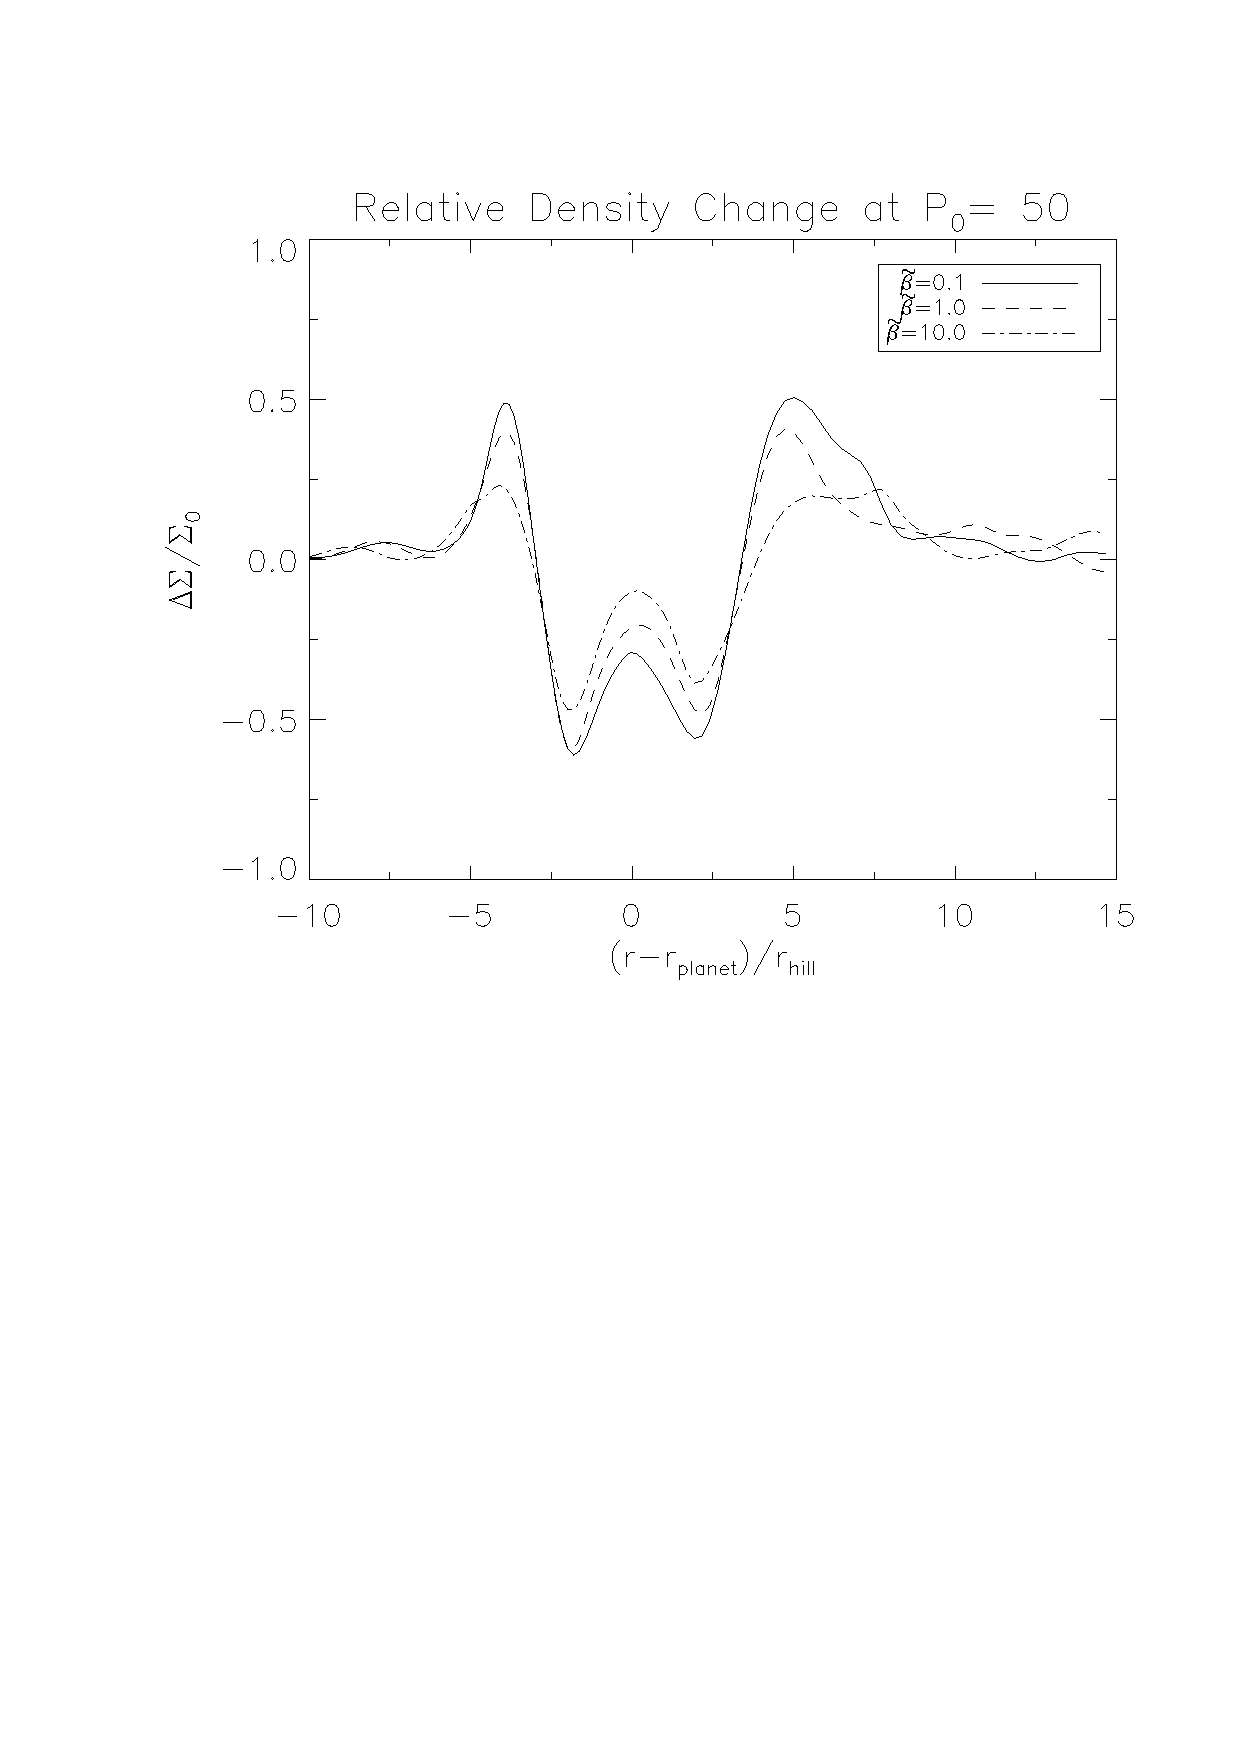
\includegraphics[width=.49\textwidth]{Posterfig_Density}\\
%           \end{minipage}
%            \hfill
%            \begin{minipage}{0.49\textwidth}
              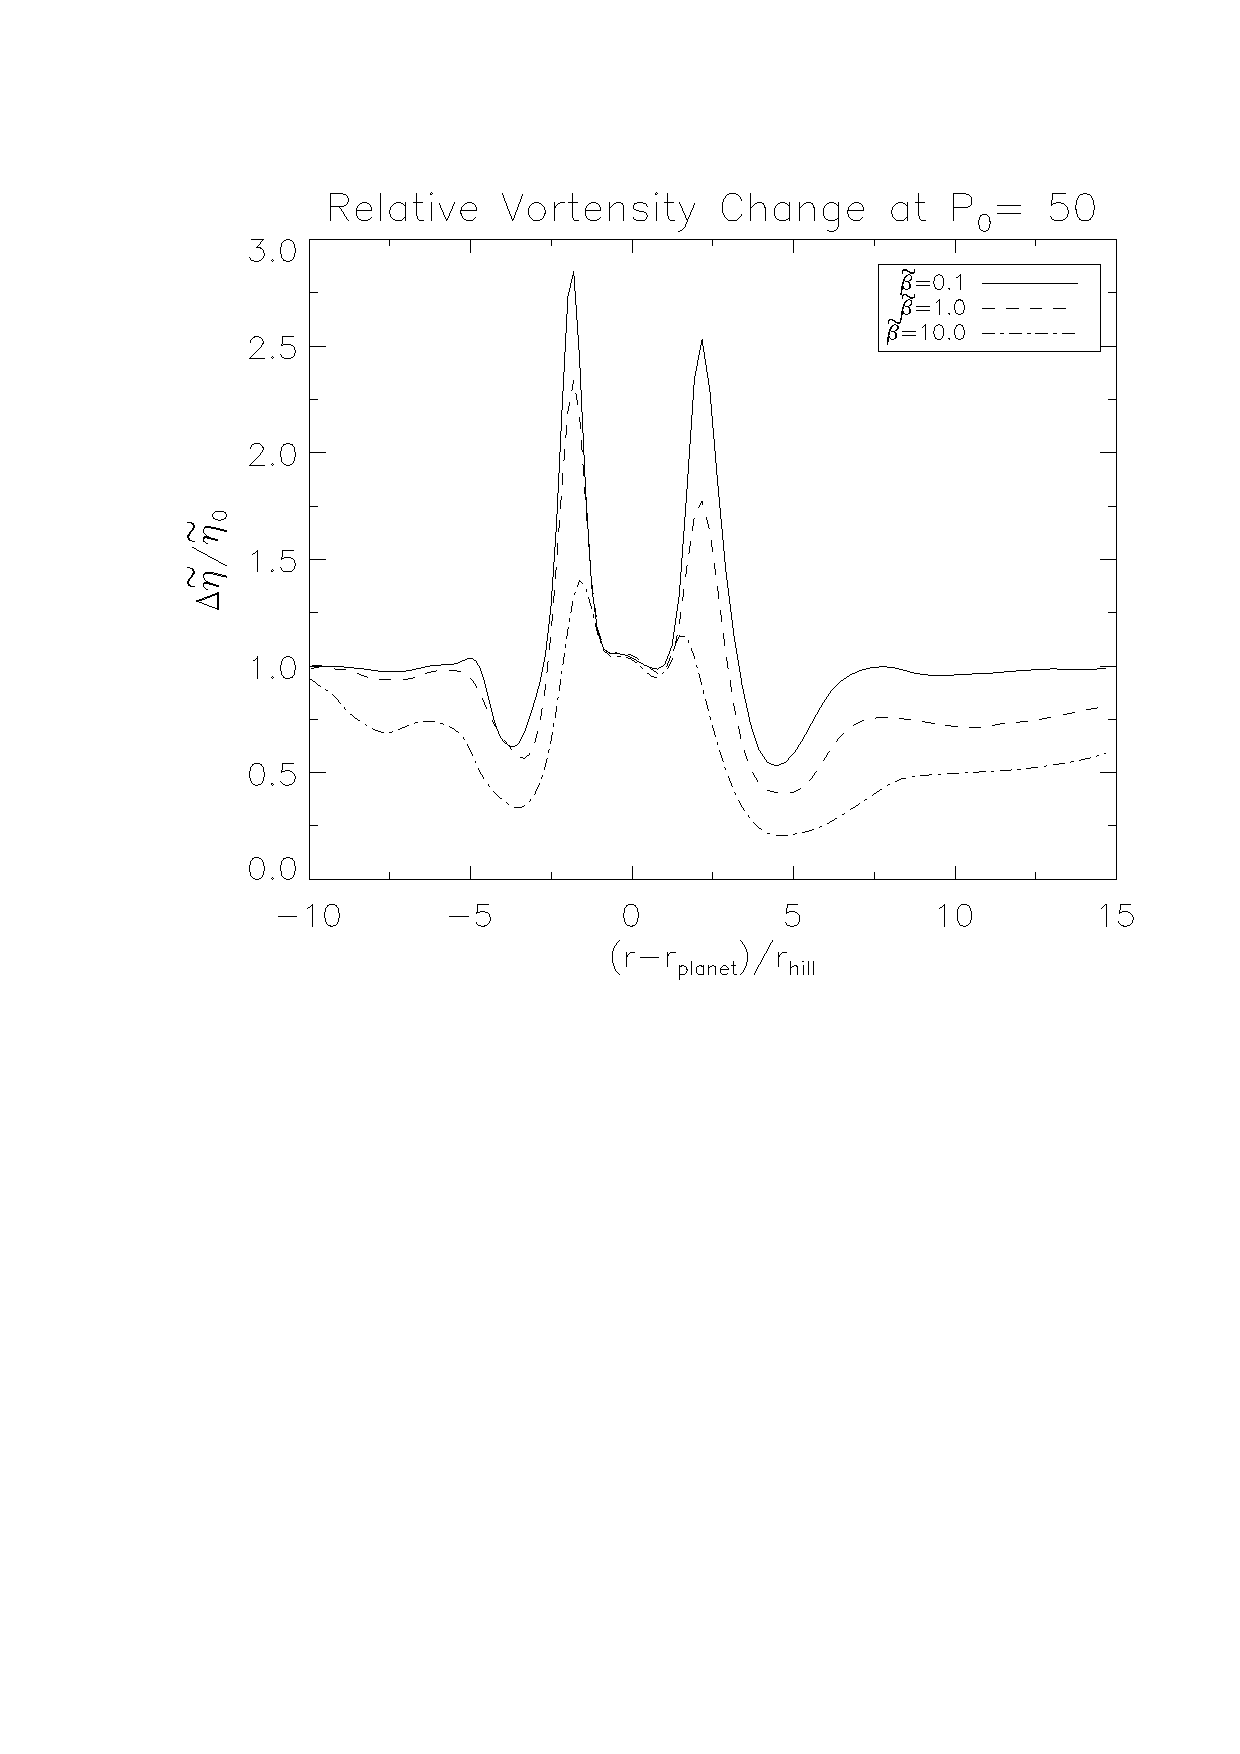
\includegraphics[width=.49\textwidth]{Posterfig_Vortensity}
%            \end{minipage}
%            \hfill
          \end{figure}
          
          %\begin{figure}
          %  \centering
          %  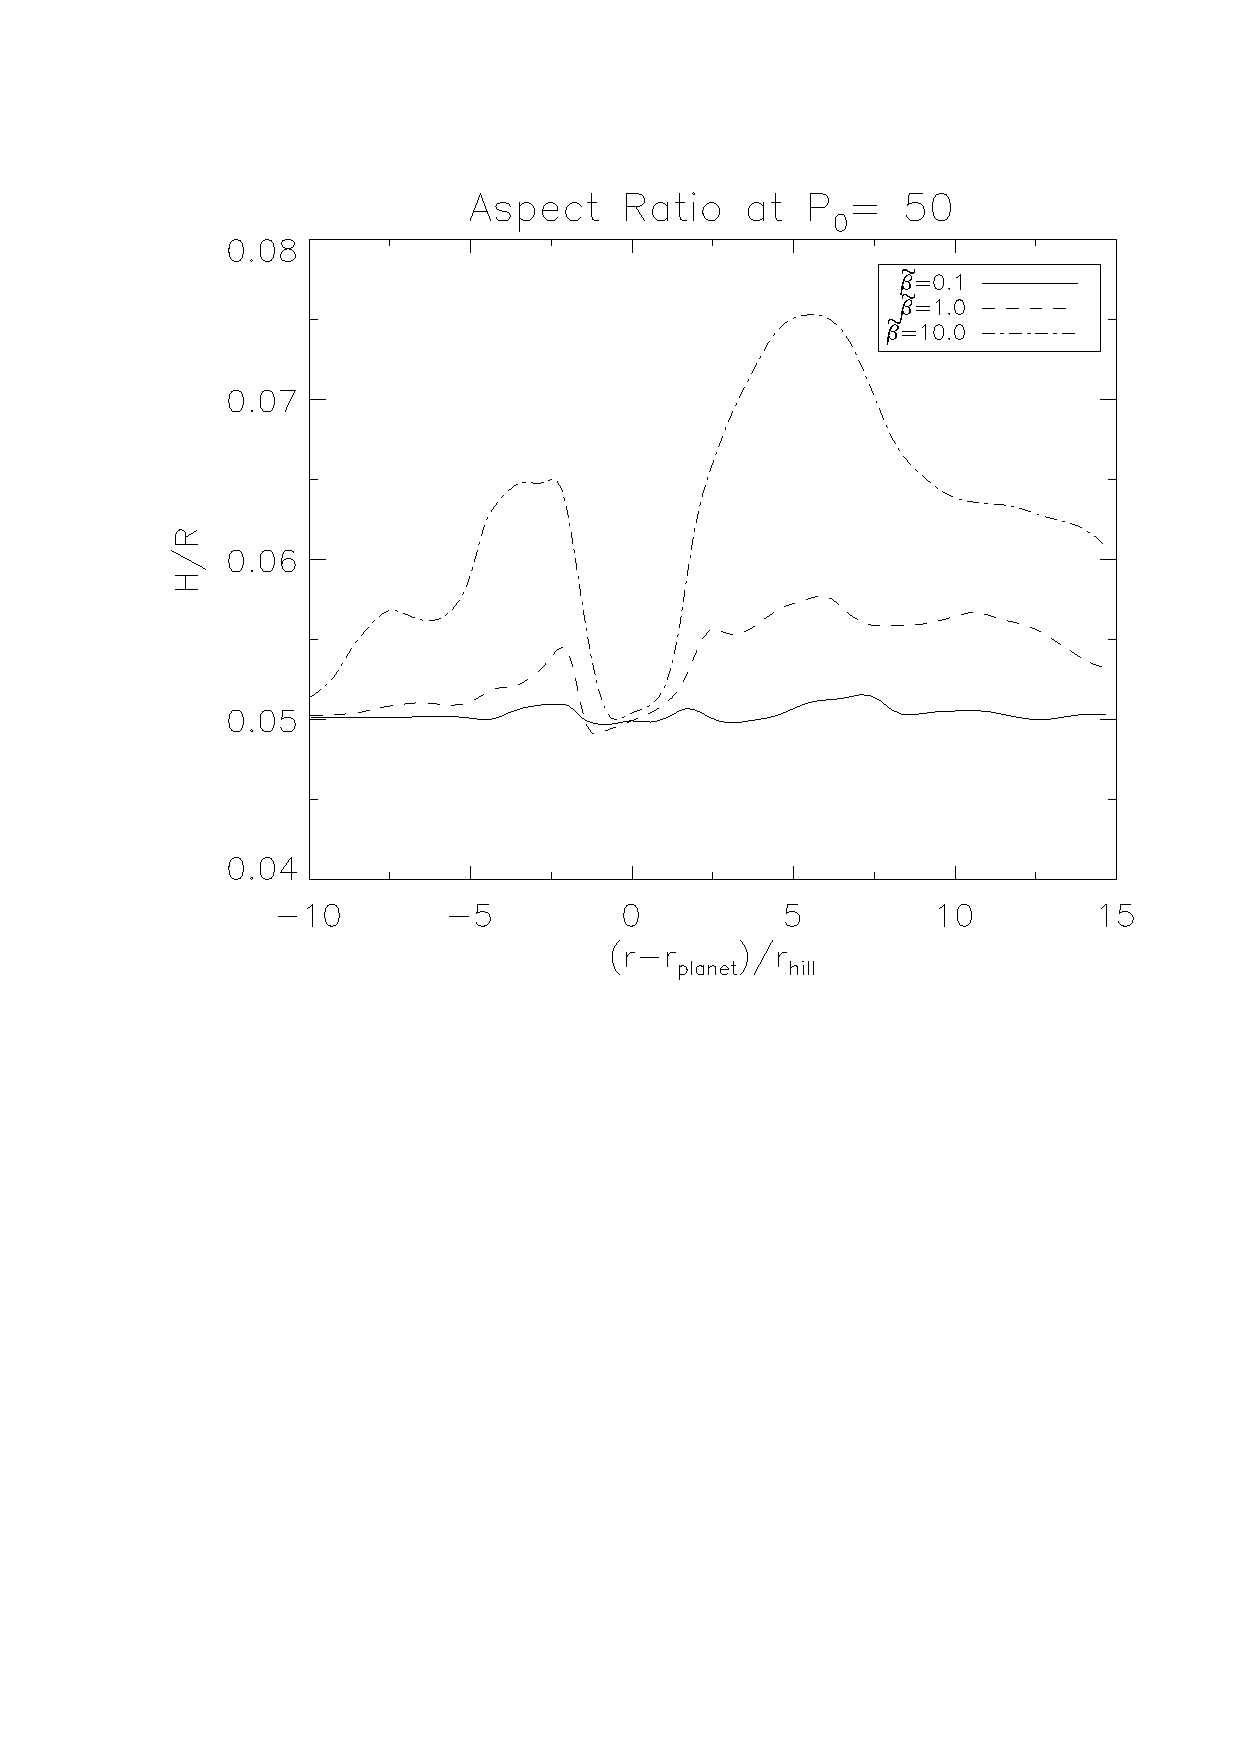
\includegraphics[width=0.5\textwidth]{Posterfig_HR}
          %\end{figure}
          
        \end{block}
        



        \vfill

            \begin{block}{{\Large Linear stability}}
              \justifying
                  {\bf plot of growth rate v.s m for different beta,
                    or table. 2D density plot showing development of
                    vortex, for different beta}

                   \begin{figure}
                    \centering
                    \hfill
                    \begin{minipage}{0.45\textwidth}
                      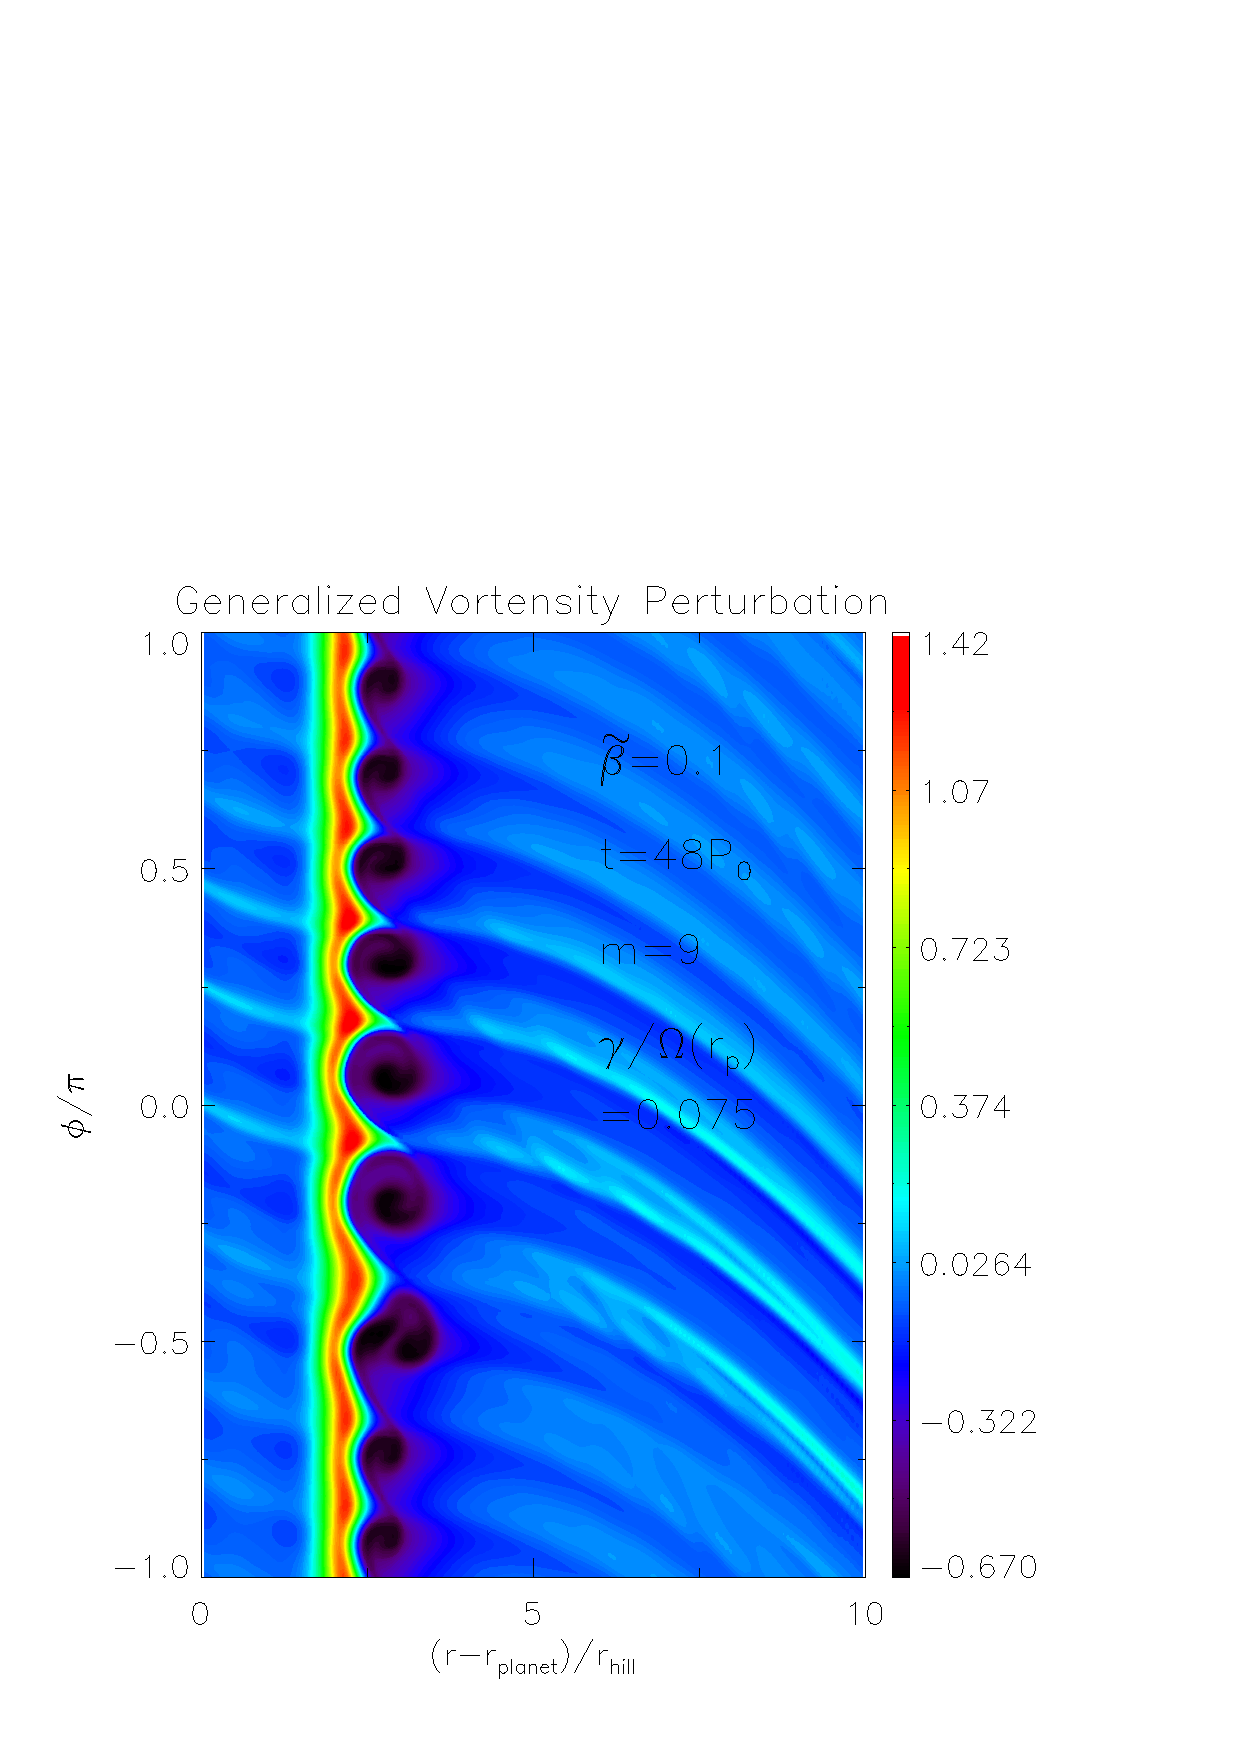
\includegraphics[width=\textwidth]{Posterfig_lowb}
                    \end{minipage}
                    \hfill
                    \begin{minipage}{0.45\textwidth}
                      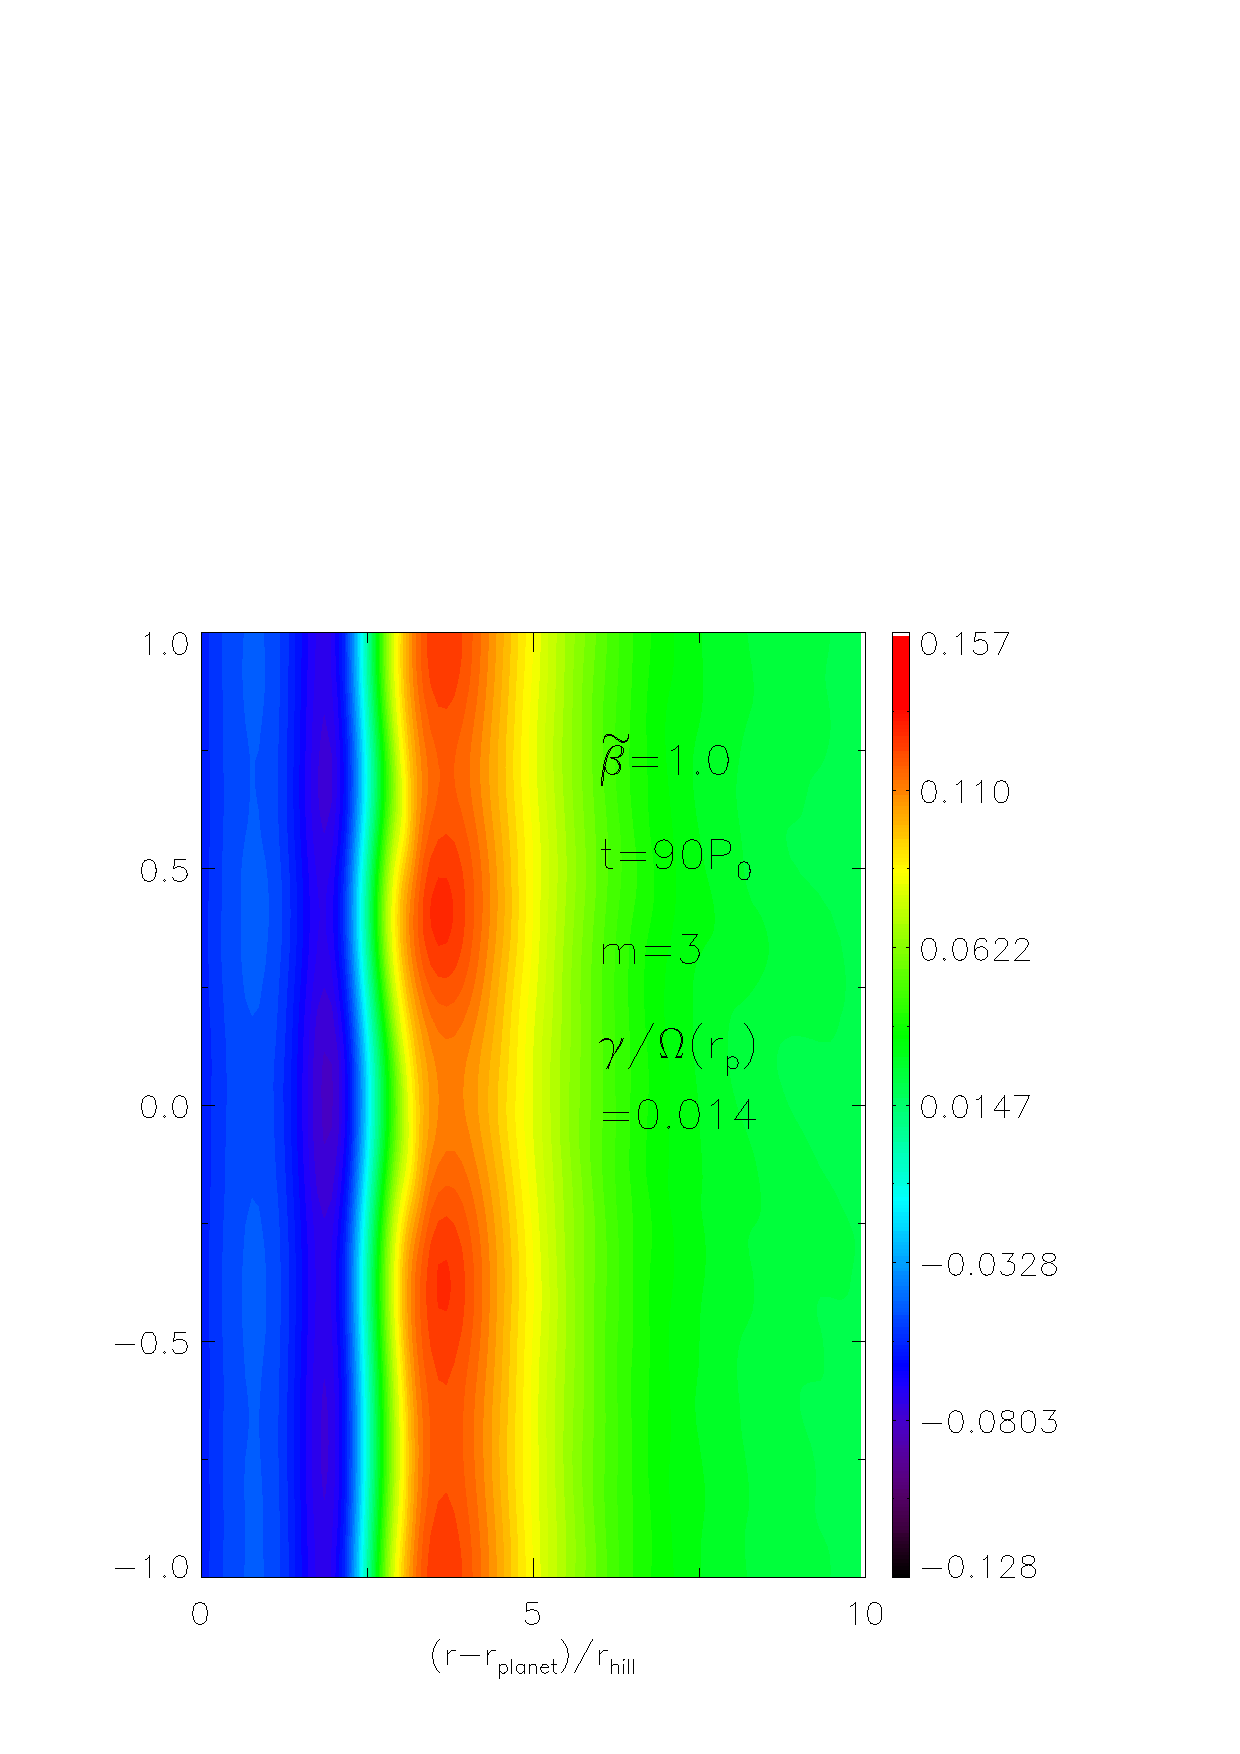
\includegraphics[width=\textwidth]{Posterfig_medb}
                    \end{minipage}
                    \hfill
                  \end{figure}

                   \begin{table}
                     \hfill
                     \begin{minipage}{\textwidth}
                       \begin{tabularx}{\textwidth}{l*{10}{R}} %\toprule \addlinespace[10pt]
                         \multicolumn{11}{c}{$\tilde{\beta}=0.1$} \\ \midrule
                         m                    & 1 & 2 & 3 & 4 & 5 & 6 & 7 & 8 & 9 & 10  \\ 
                         $\gamma10^2/\Omega(r_o)$ & 6.56 & 6.82 & 6.73 & 5.78 & 6.00 & 6.38 & 5.97 & 5.62 & 4.61 & 3.36   \\ \bottomrule
                       \end{tabularx}
                     \end{minipage}

                     \vspace{1in}

                     \begin{minipage}{\textwidth}
                       \begin{tabularx}{\textwidth}{l*{5}{R}} %\toprule \addlinespace[10pt]
                         \multicolumn{6}{c}{$\tilde{\beta}=1.0$} \\ \midrule
                         m                    & 1 & 2 & 3 & 4 & 5  \\ 
                         $\gamma10^2/\Omega(r_o)$ & 1.27 & 1.28 & 1.35 & 1.01 & 0.61   \\ \bottomrule
                       \end{tabularx}
                     \end{minipage}
                     \hfill
                   \end{table}

                   
            \end{block}
            \vfill
          }
        \end{minipage}
      \end{beamercolorbox}
    \end{column}
    % ---------------------------------------------------------%
    % end the column
    
    % ---------------------------------------------------------%
    % Set up a column 
    \begin{column}{.49\textwidth}
      \begin{beamercolorbox}[center,wd=\textwidth]{postercolumn}
        \begin{minipage}[T]{.95\textwidth} % tweaks the width, makes a new \textwidth
          \parbox[t][\columnheight]{\textwidth}{ % must be some better way to set the the height, width and textwidth simultaneously
            % Since all columns are the same length, it is all nice and tidy.  You have to get the height empirically
            % ---------------------------------------------------------%
            % fill each column with content
            
            \begin{block}{\Large{Linear stability Cont.}}
              \justifying
              \begin{figure}
                \centering
                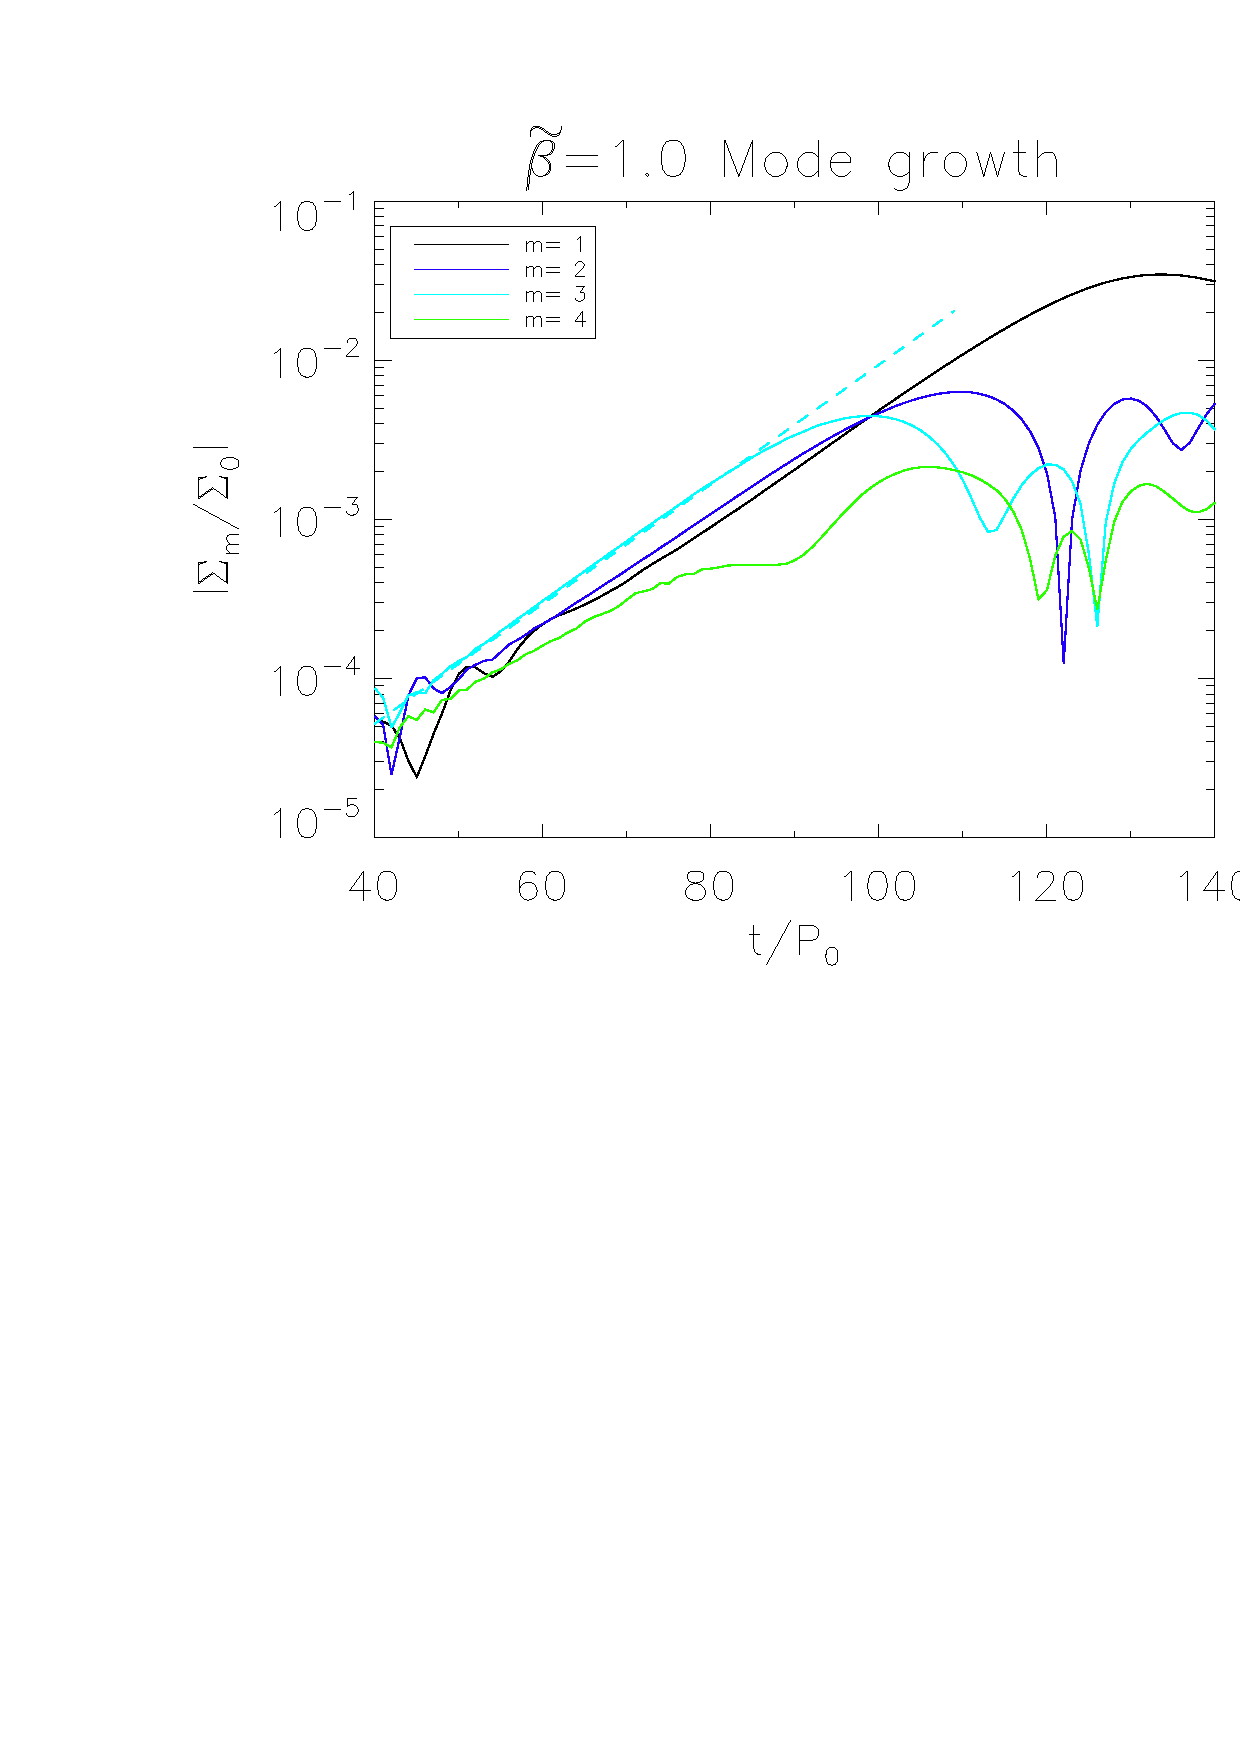
\includegraphics[width=\textwidth]{Posterfig_Growth}
              \end{figure}
            \end{block}

            \vfill

            \begin{block}{\Large{Non-linear vortex evolution}}
              \justifying
                  {\bf `lifetime' plot of m=1 for diff beta, snapshots
                    (before, during, after vortex decay). quote rossby
                  number when vortices in quasi-steady state}

                  \begin{figure}
                    \centering
                    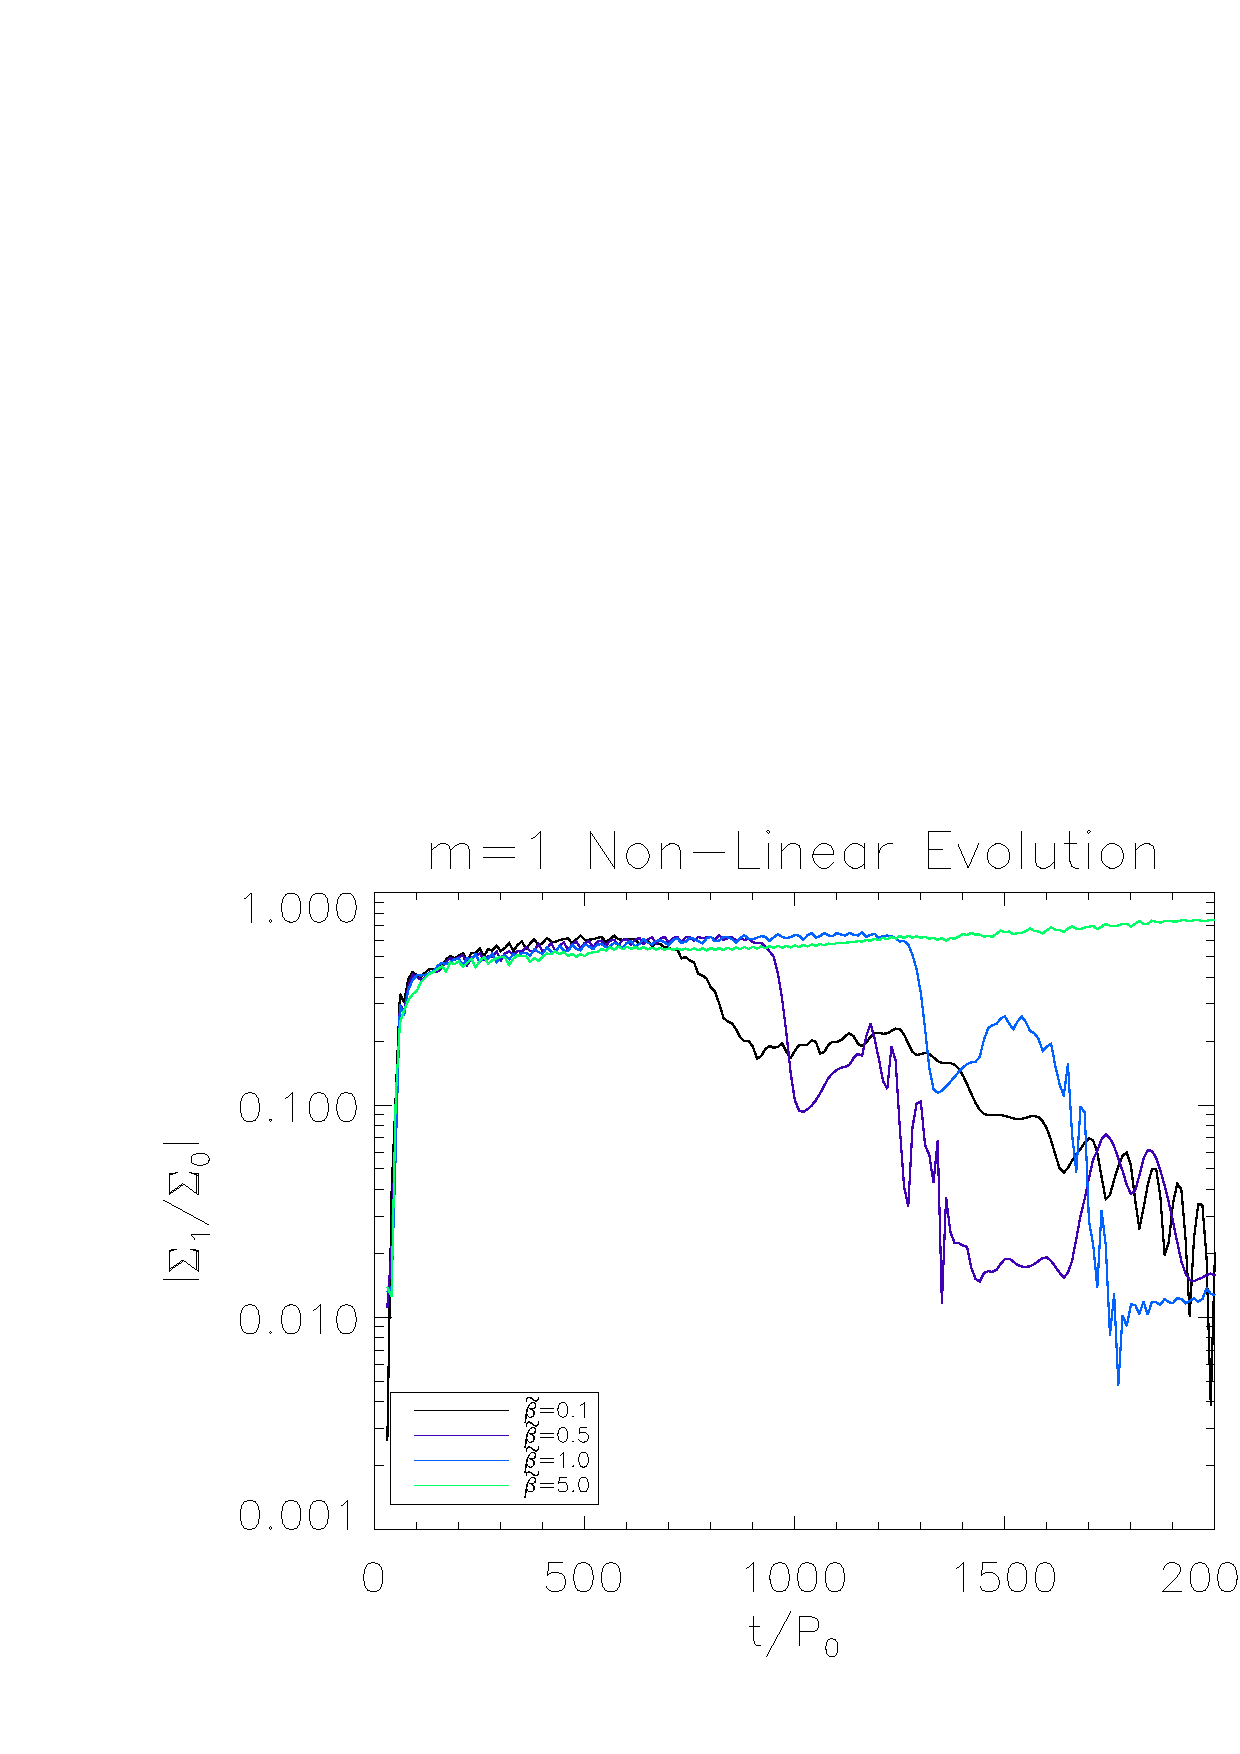
\includegraphics[width=\textwidth]{Posterfig_Lifetime_b}
                  \end{figure}

                  \begin{figure}
                    \centering
                    \hfill
                    \begin{minipage}{0.3\textwidth}
                      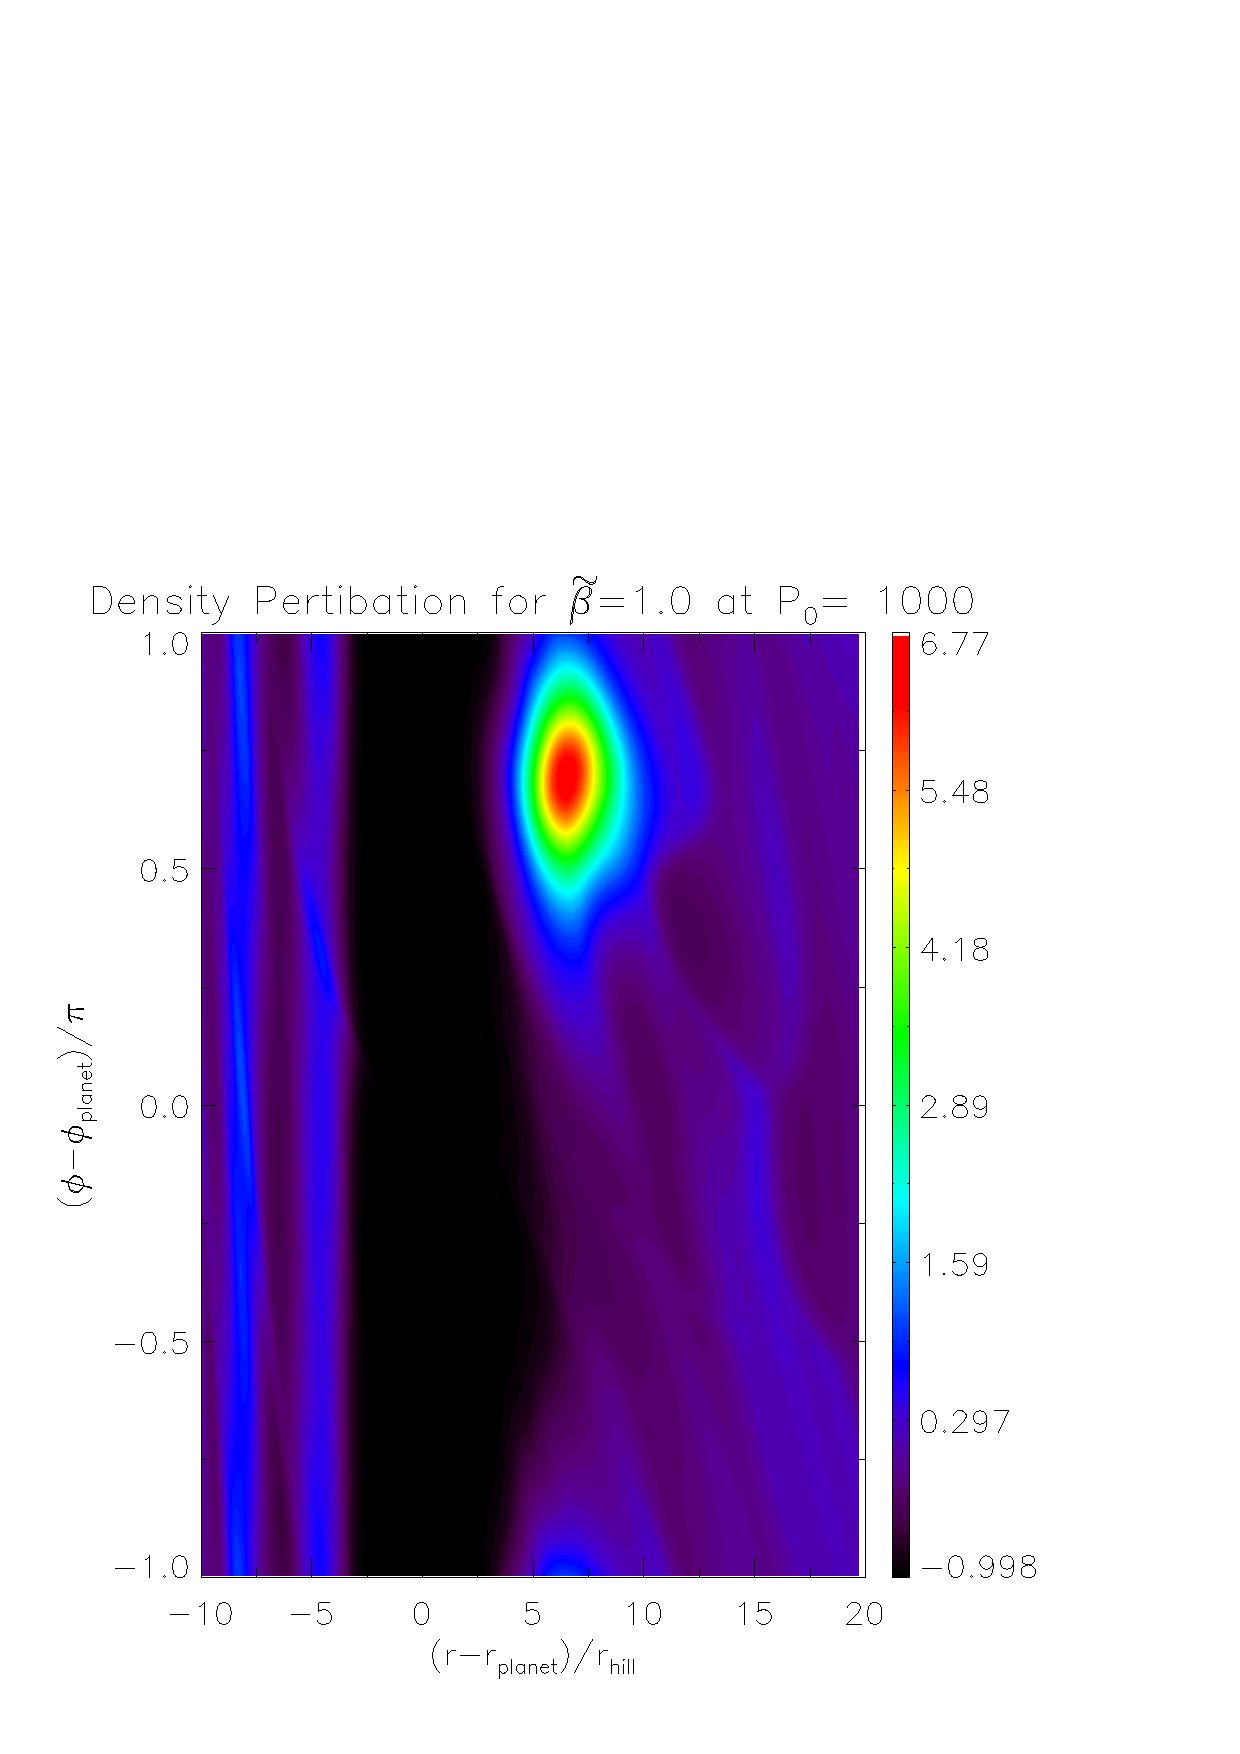
\includegraphics[width=\textwidth]{Posterfig_Before}
                      \caption{$Ro=-0.16$}
                    \end{minipage}
                    \hfill
                    \begin{minipage}{0.3\textwidth}
                      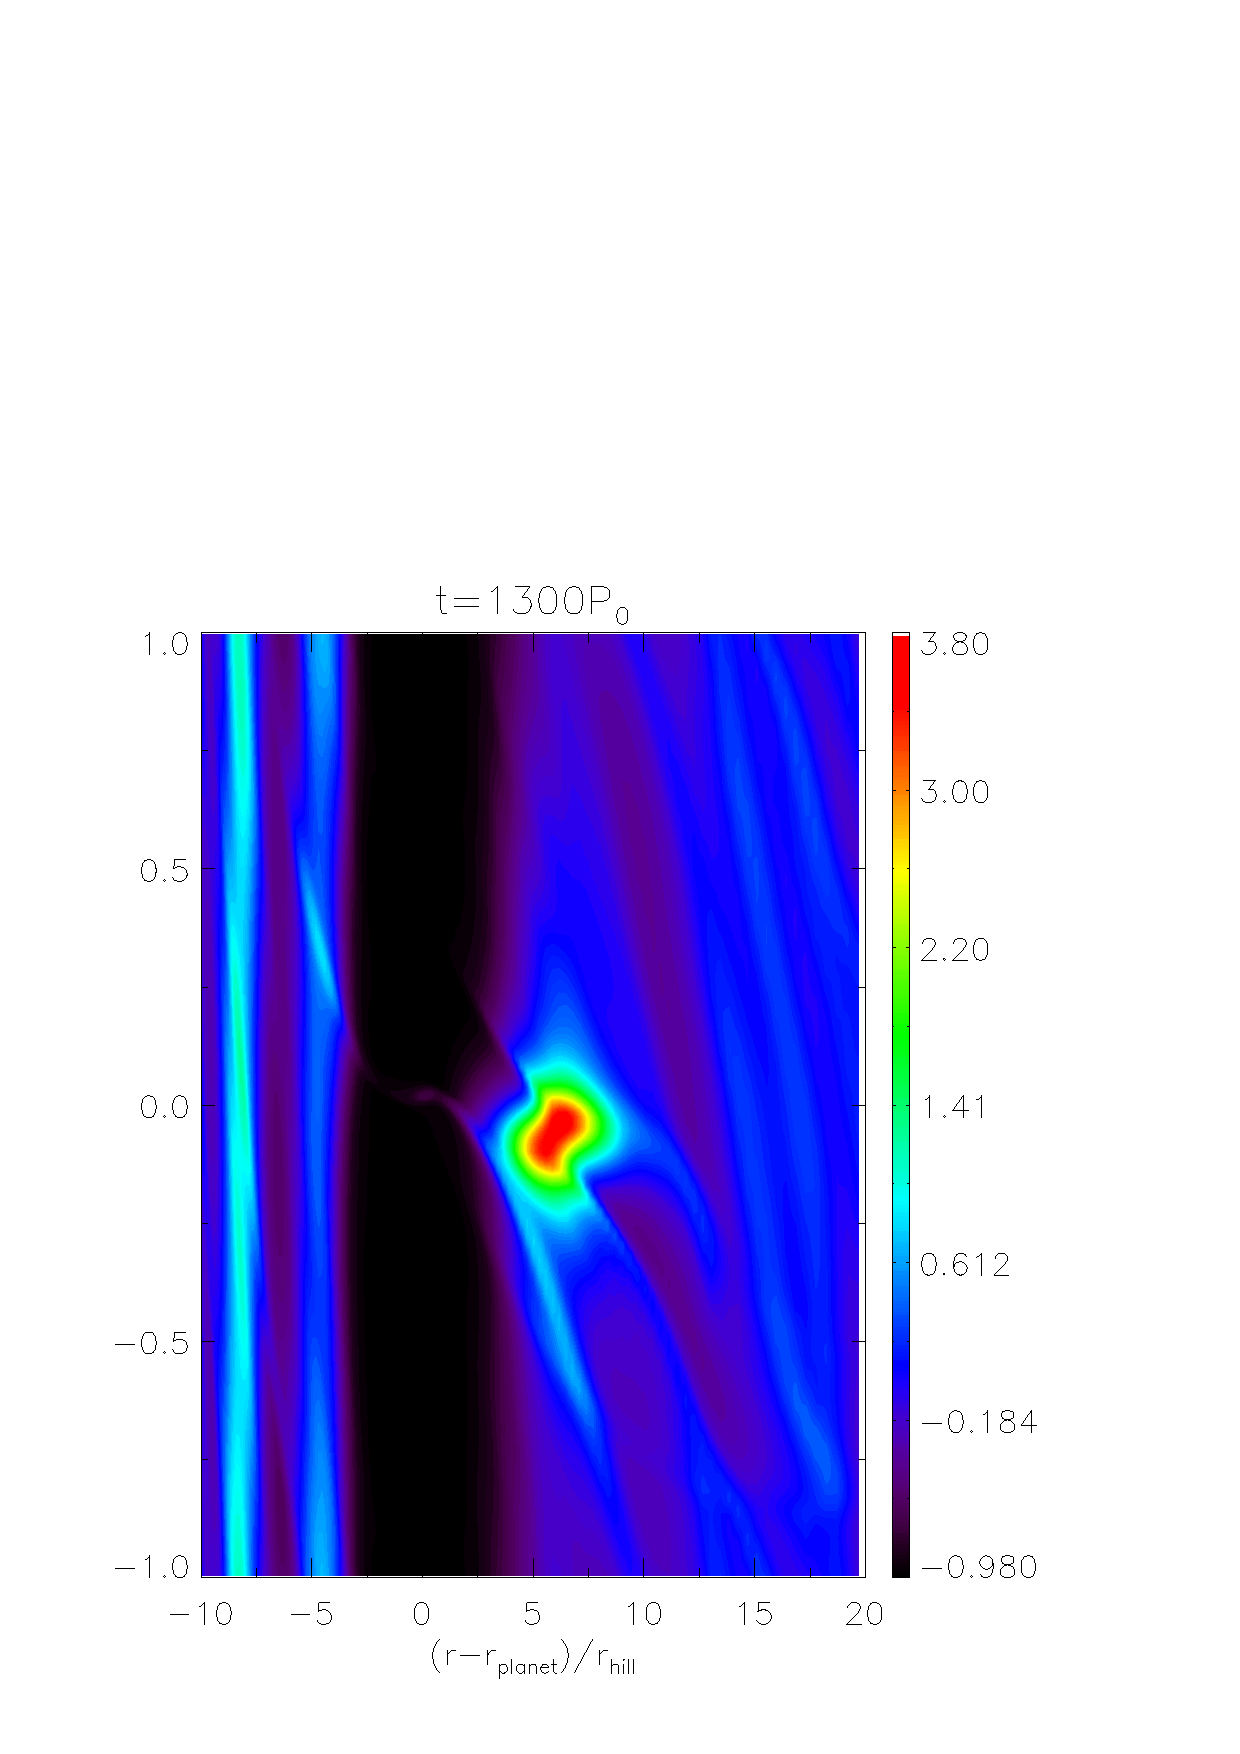
\includegraphics[width=\textwidth]{Posterfig_During}
                      \caption{$Ro=-0.43$}
                    \end{minipage}
                    \hfill
                    \begin{minipage}{0.3\textwidth}
                      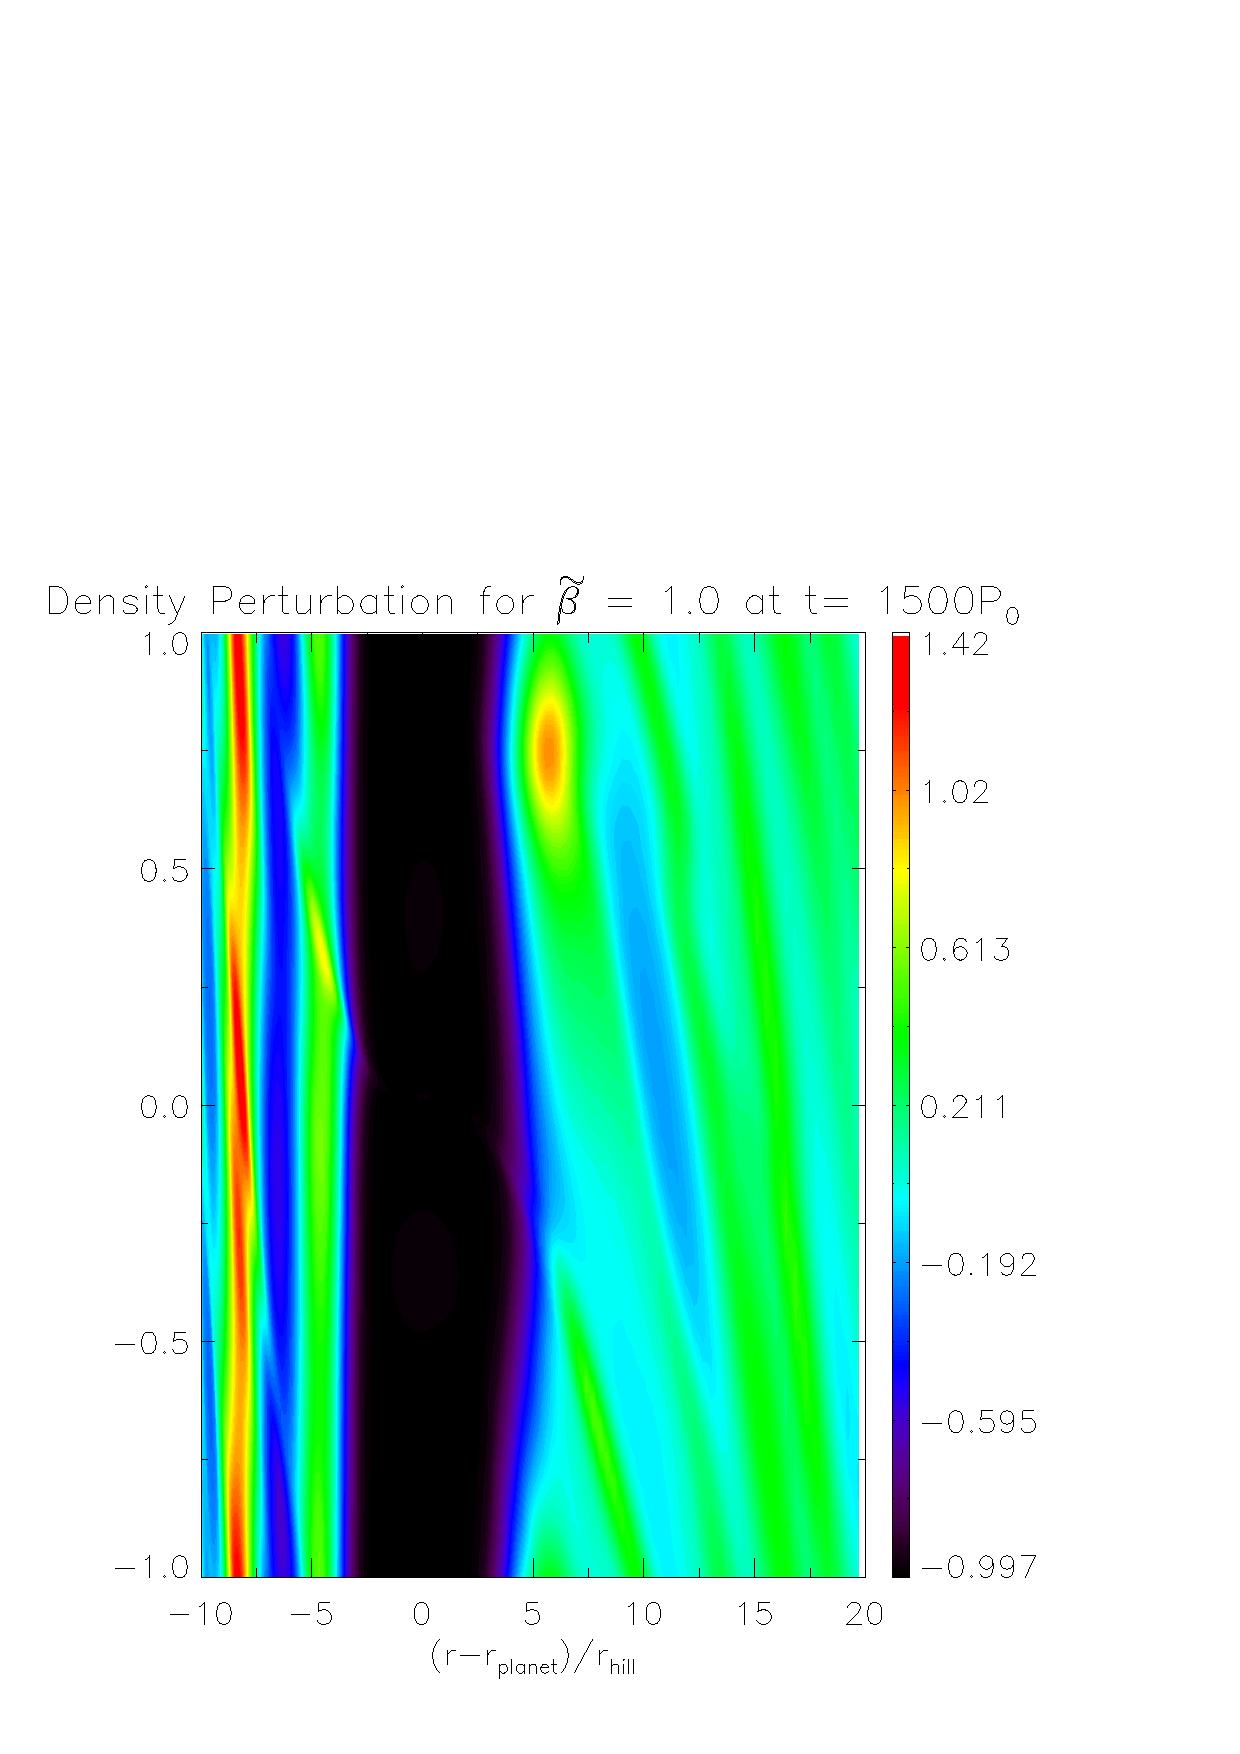
\includegraphics[width=\textwidth]{Posterfig_After}
                      \caption{$Ro=-0.10$}
                    \end{minipage}
                    \hfill
                  \end{figure}

            \end{block}
            \vfill
    
            \begin{block}{{\Large Conclusions so far}}\justifying
              {\large{\bf
                  
                }
              }
              \vfill
            \end{block}
          }
          % ---------------------------------------------------------%
          % end the column
        \end{minipage}
      \end{beamercolorbox}
    \end{column}
    % ---------------------------------------------------------%
    % end the column
  \end{columns}
  \vskip1ex
  %\tiny\hfill\textcolor{ta2gray}{Created with \LaTeX \texttt{beamerposter}  \url{http://www-i6.informatik.rwth-aachen.de/~dreuw/latexbeamerposter.php}}
  %% \tiny\hfill{Created with \LaTeX \texttt{beamerposter}  \url{http://www-i6.informatik.rwth-aachen.de/~dreuw/latexbeamerposter.php} \hskip1em}
\end{frame}
\end{document}


%%%%%%%%%%%%%%%%%%%%%%%%%%%%%%%%%%%%%%%%%%%%%%%%%%%%%%%%%%%%%%%%%%%%%%%%%%%%%%%%%%%%%%%%%%%%%%%%%%%%
%%% Local Variables: 
%%% mode: latex
%%% TeX-PDF-mode: t
%%% End:
